% Please make sure you insert your
% data according to the instructions in PoSauthmanual.pdf
\documentclass[a4paper,11pt]{article}
\usepackage{pos}
\usepackage{xspace}
\usepackage{subcaption}

\title{Euclid: Sensitivity to Neutrino Parameters}
%% \ShortTitle{Short Title for header}

\newcommand{\euclid}{\textit{Euclid}\xspace}
\newcommand{\planck}{\textit{Planck}\xspace}

\newcommand{\dneff}{\Delta N_\mathrm{eff}}
\newcommand{\summnu}{\sum m_\nu}

\newcommand{\threetimestwo}{3$\times$2\,pt}

\newcommand{\camb}{\texttt{CAMB}\xspace}
\newcommand{\class}{\texttt{CLASS}\xspace}
\newcommand{\montepython}{\texttt{MontePython}\xspace}
\newcommand{\cosmicfish}{\texttt{CosmicFish}\xspace}

\author[1,2]{ M.~Archidiacono}
\author[3]{ J.~Lesgourgues}
\author[3]{ S.~Casas}
\author*[4]{ S.~Pamuk}
\author[5]{ N.~Sch\"oneberg}
\author[6,7,8]{ Z.~Sakr}
\author[9,10,11]{ G.~Parimbelli}
\author[12]{ A.~Schneider}
\author[13,12]{ F.~Hervas~Peters}
\author[14,15,16]{ F.~Pace}
\author[3,17]{ V.~M.~Sabarish}
\author[18,19,20]{ M.~Costanzi}
\author[14,15,16]{ S.~Camera}
\author[21]{ C.~Carbone}
\author[22]{ S.~Clesse}
\author[23]{ N.~Frusciante}
\author[24,20]{ A.~Fumagalli}
\author[18,19,25,20]{ P.~Monaco}
\author[26]{ D.~Scott}
\author[19,18,10,24,27]{ M.~Viel}

\affiliation[1]{Dipartimento di Fisica "Aldo Pontremoli", Universit\`a degli Studi di Milano, Via Celoria 16, 20133 Milano, Italy}
\affiliation[2]{INFN-Sezione di Milano, Via Celoria 16, 20133 Milano, Italy}
\affiliation[3]{Institute for Theoretical Particle Physics and Cosmology (TTK), RWTH Aachen University, 52056 Aachen, Germany}
\affiliation[4]{Instituto de F\'{\i}sica de Cantabria (IFCA), CSIC-Univ. de Cantabria, Avda. de los Castros s/n, E-39005 Santander, Spain}
\affiliation[5]{Institut de Ci\`{e}ncies del Cosmos (ICCUB), Universitat de Barcelona (IEEC-UB), Mart\'{i} i Franqu\`{e}s 1, 08028 Barcelona, Spain}
\affiliation[6]{Institut f\"ur Theoretische Physik, University of Heidelberg, Philosophenweg 16, 69120 Heidelberg, Germany}
\affiliation[7]{Institut de Recherche en Astrophysique et Plan\'etologie (IRAP), Universit\'e de Toulouse, CNRS, UPS, CNES, 14 Av. Edouard Belin, 31400 Toulouse, France}
\affiliation[8]{Universit\'e St Joseph; Faculty of Sciences, Beirut, Lebanon}
\affiliation[9]{Institute of Space Sciences (ICE, CSIC), Campus UAB, Carrer de Can Magrans, s/n, 08193 Barcelona, Spain}
\affiliation[10]{Dipartimento di Fisica, Universit\`a degli studi di Genova, and INFN-Sezione di Genova, via Dodecaneso 33, 16146, Genova, Italy}
\affiliation[11]{SISSA, International School for Advanced Studies, Via Bonomea 265, 34136 Trieste TS, Italy}
\affiliation[12]{Department of Astrophysics, University of Zurich, Winterthurerstrasse 190, 8057 Zurich, Switzerland}
\affiliation[13]{AIM, CEA, CNRS, Universit\'{e} Paris-Saclay, Universit\'{e} de Paris, 91191 Gif-sur-Yvette, France}
\affiliation[14]{Dipartimento di Fisica, Universit\`a degli Studi di Torino, Via P. Giuria 1, 10125 Torino, Italy}
\affiliation[15]{INFN-Sezione di Torino, Via P. Giuria 1, 10125 Torino, Italy}
\affiliation[16]{INAF-Osservatorio Astrofisico di Torino, Via Osservatorio 20, 10025 Pino Torinese (TO), Italy}
\affiliation[17]{Hamburger Sternwarte, University of Hamburg, Gojenbergsweg 112, 21029 Hamburg, Germany}
\affiliation[18]{Dipartimento di Fisica - Sezione di Astronomia, Universit\`a di Trieste, Via Tiepolo 11, 34131 Trieste, Italy}
\affiliation[19]{INAF-Osservatorio Astronomico di Trieste, Via G. B. Tiepolo 11, 34143 Trieste, Italy}
\affiliation[20]{IFPU, Institute for Fundamental Physics of the Universe, via Beirut 2, 34151 Trieste, Italy}
\affiliation[21]{INAF-IASF Milano, Via Alfonso Corti 12, 20133 Milano, Italy}
\affiliation[22]{Universit\'e Libre de Bruxelles (ULB), Service de Physique Th\'eorique CP225, Boulevard du Triophe, 1050 Bruxelles, Belgium}
\affiliation[23]{Department of Physics "E. Pancini", University Federico II, Via Cinthia 6, 80126, Napoli, Italy}
\affiliation[24]{Ludwig-Maximilians-University, Schellingstrasse 4, 80799 Munich, Germany}
\affiliation[25]{INFN, Sezione di Trieste, Via Valerio 2, 34127 Trieste TS, Italy}
\affiliation[26]{Department of Physics and Astronomy, University of British Columbia, Vancouver, BC V6T 1Z1, Canada}
\affiliation[27]{ICSC - Centro Nazionale di Ricerca in High Performance Computing, Big Data e Quantum Computing, Via Magnanelli 2, Bologna, Italy}

\emailAdd{pamuk@ifca.unican.es}

\abstract{The European Space Agency has launched its newest mission in July 2023. The Euclid mission is planned to create one of the largest galaxy clustering and weak gravitational lensing survey to its date. The complimentary of a wide photometric redshift galaxy survey and spectroscopic survey will provide excellent sensitivity to the history of structure foramtion.\\
The following presents the newest forecast of \euclid done within the collaboration for the mission's main cosmological probes to see how well future data from \euclid will be able to constrain parameters from Neutrino physics. This forecast is focused on the summed mass of neutrino species $\summnu$, as well as the effective number of additional ultra relativistic species $\dneff$.\\
We show how the upcoming data could lead to unprecedented sensitivity in these parameters and could, together with data from future cosmic microwave background experiments, be able to have a detection of the neutrino mass scale.}

\FullConference{12th Neutrino Oscillation Workshop (NOW2024)\\
 2-8, September 2024\\
Otranto, Lecce, Italy\\}

%% \tableofcontents

\begin{document}
\maketitle


\section{Background}
The \euclid mission\cite{euclidcollaboration2024euclidiovervieweuclid} will measure the location and shape of close to a billion galaxies over approximately one-third of the sky. With a look back time of roughly ten billion years, \euclid will produce the largest galaxy catalogue to date. The cosmological information that can be obtained from this can be used to measure the cosmological neutrino mass, $\sum m_\nu$, as well as the effective number of additional ultra-relativistic relics, $\Delta N_\mathrm{eff}$.\\
The effect of these quantities on cosmological observables is described in \cite{ParticleDataGroup:2024cfk, Vagnozzi_2018, ISTF2020}. In the following section, we will briefly introduce these observables.

The observable that is mainly constraining the cosmological neutrino mass is the weak lensing (WL) probe.
The shapes of background (source) galaxies correlate with each other as they are lensed by the same foreground (lens) galaxies. This correlation can be directly related to the correlation of the underlying matter field. Adding massive neutrinos suppresses this correlation in a scale-dependent way, as it slows down the formation of structure for scales that enter the Hubble horizon while neutrinos are still too hot to cluster inside gravitational wells. Measuring the WL signal gives a unique method to directly measure the overall amplitude of the matter perturbations   

The probe most strongly constraining $\dneff$ is Galaxy clustering (GC), where we measure the spatial correlation of galaxies. The two-point correlation function shows an excess at a particular scale, originating from expanding acoustic waves in the primordial plasma. The angular size of these baryonic acoustic oscillations (BAO) is determined by the universe's expansion history. This is why adding additional massless relics through $\dneff$ creates a measurable signal in the BAO.

Additionally to the BAO, the amplitude of the GC signal is also given by the underlying matter distribution. As galaxies form in over-dense regions an over density in the galaxy     distribution is related to the over density in the total matter. Contrary the the WL signal this relation is not a direct correspondence, rather the galaxy field is a biased tracer of the galaxy field. On its own, the GC probe could only be able to measure the amplitude of matter perturbations in combination with proportionality constants called galaxy biases. \euclid will be able to construct the GC power spectrum using photometric redshifts, as well using spectroscopic ones. While the galaxies for which we have measured photometric redshifts will mainly be used after binning them in tomographic redshift bins, the spectroscopic redshift measurements will allow for the computation of the three-dimensional redshift space power spectrum. The latter additionally considers redshift space distortions(RSD). We denote these two probes as GCph and GCsp respectively.

The combination of the WL and GC probe can be used to break degeneracies as they measure different tracers (gravitational potential and clustered matter respectively), which are differently affected by $\dneff$ and $\summnu$. Given that the intervening lenses for WL are mostly clustered galaxies, it is natural to expect a cross-correlation (XC) between the WL and GCph probes. From these probes, we construct two-point statistics.

Additionally to these probes, we add information from the cosmic microwave background (CMB) to further constrain neutrino parameters and break possible degeneracies.

\section{Methodology}

The forecast is done using Markov chain Monte Carlo (MCMC) methods to go beyond the standard Fisher information (FI) formalism. This is done, as we expect deviations from Gaussian posteriors for the neutrino parameters, as well as to add the physical constraints of a positive neutrino mass.

The validation of our forecast was done in 3 separate steps. In the first step, we validated our Einstein--Boltzmann solver (EBS) by performing multiple FI forecasts where we have compared different EBSs. For this forecast, we used the \cosmicfish code that was validated before within the efforts of the Euclid consortium\cite{ISTF2020}. The two most common EBSs are \camb\cite{2011ascl.soft02026L} and \class\cite{Diego_Blas_2011}. While their agreement has been established for past CMB and LSS experiments, the new frontier of precision unlocked by \euclid required a new validation at higher precision requirements. Furthermore, the \euclid observables will need us to have a good handle on the non-linear corrections to the power spectrum. We performed a thorough analysis of multiple recipes for these non-linear corrections and compared them to N-body simulations. In the presence of massive neutrinos, the best comparison was achieved with the \texttt{HMCode2020} recipe \cite{Mead_2021}. Like this, the \texttt{HMCode2020} recipes within \class and \camb were validated for the first time.

We then formulated a likelihood for \montepython\cite{Audren:2012wb} as an extension of the existing likelihood formulated in \cite{casas2023euclidvalidationmontepythonforecasting}. The modelling of the galaxy bias needs particular care in the presence of massive neutrinos. Else this can bias the measured value and sensitivity for $\summnu$ \cite{Vagnozzi_2018}. As neutrinos did not cluster inside halos, the RSD is also driven by cold dark matter and baryonic matter only\cite{Villaescusa_Navarro_2018}. For this reason, the measured signal has to be additionally modified to describe this defect. In the second step, We validated our likelihood by performing a FI forecast with it. We compare the results to the ones of the first step.

Finally, we ran an MCMC using our \montepython likelihood to check for the validity of our FI forecast. We observed deviations between MCMC and FI that could be explained by non-Gaussianities of the posterior as well as from prior effects. This confirms the need of using MCMC methods. 

\section{Results}

The final forecast was performed using \montepython. We decided to vary different sets of cosmological parameters for the analysis to study how much the constraints degrade by opening up the parameter space. The baseline model consists of  five $\varLambda$CDM parameters as well as $\summnu$ (i.e $h, \Omega_\mathrm{m}, \Omega_\mathrm{b}, \sigma_8, n_\mathrm{s}, \summnu$). We also studied what happens when opening up the number of additional massless relics $\{\dneff\}$, and/or the Chevallier--Polarski--Linder parameters for the equation of state of dark energy $\{w_0,w_a\}$. Additionally, when adding information from CMB experiments we vary the optical depth of reionisation $\tau$. We assume flat cosmology and three massive neutrinos with degenerate masses. It was shown that the latter choice is appropriate as individual mass splittings are not resolvable with cosmological data\cite{Lesgourgues:2013sjj}.

We performed these forecasts for different combinations of the \euclid main probes as well as adding additional information from CMB experiments. For the survey specifications of \euclid we stick to the pessimistic settings outlined in \cite{ISTF2020}. We consider two cases for the CMB experiments: We either use a mock likelihood for \planck or for a more futuristic setup of CMB-S4 + LiteBird.

For the combination of the main \euclid probes we find in the baseline model a sensitivity to the cosmological neutrino mass of $\sigma\left(\summnu\right) = 56\,\mathrm{meV}$. This degrades to a 95\% confidence level (CL) of $\summnu<220\,\mathrm{meV}$ when opening up $\dneff$. The distribution is non-Gaussian due to the prior edge, and therefore we report the upper bound. For $\dneff$ we find an upper bound of $\dneff<0.746$ at a 95\% CL. Additionally opening up the dark energy equation of state does not measurably degrade the sensitivity to $\summnu$ while the 95\% CL of $\dneff$ degrades to $\dneff<0.935$.  

Adding CMB to this tightens the constraints in the full ten-parameter model to $\sigma\left(\summnu\right) = 40\,\mathrm{meV}$ or $\sigma\left(\summnu\right) = 31\,\mathrm{meV}$ for \planck or CMB-S4+LiteBird respectively. The constraints on $\dneff$ are dominated by CMB probes but the main degeneracy of $\dneff$ with the reduced Hubble constant $h$ is broken through the \euclid data. The combination of \euclid and CMB data could provide unprecedented sensitivity to $\dneff$ with a forecast sensitivity of $\dneff<0.149$ or $\dneff<0.069$ for \euclid + \planck or \euclid + CMB-S4 + LiteBird respectively. 

The forecast sensitivities are put in a physical context in Figure \ref{fig:results}. We show how for the minimal mass scenario \euclid + CMB could be able to put the inverted hiracy models into tension. Additionally, this combination will be able to exclude the most common types of dark relics with pre-QCD injections.   

\begin{figure}[!htbp]
    \centering
    \begin{subfigure}{0.49\textwidth}
        \centering
        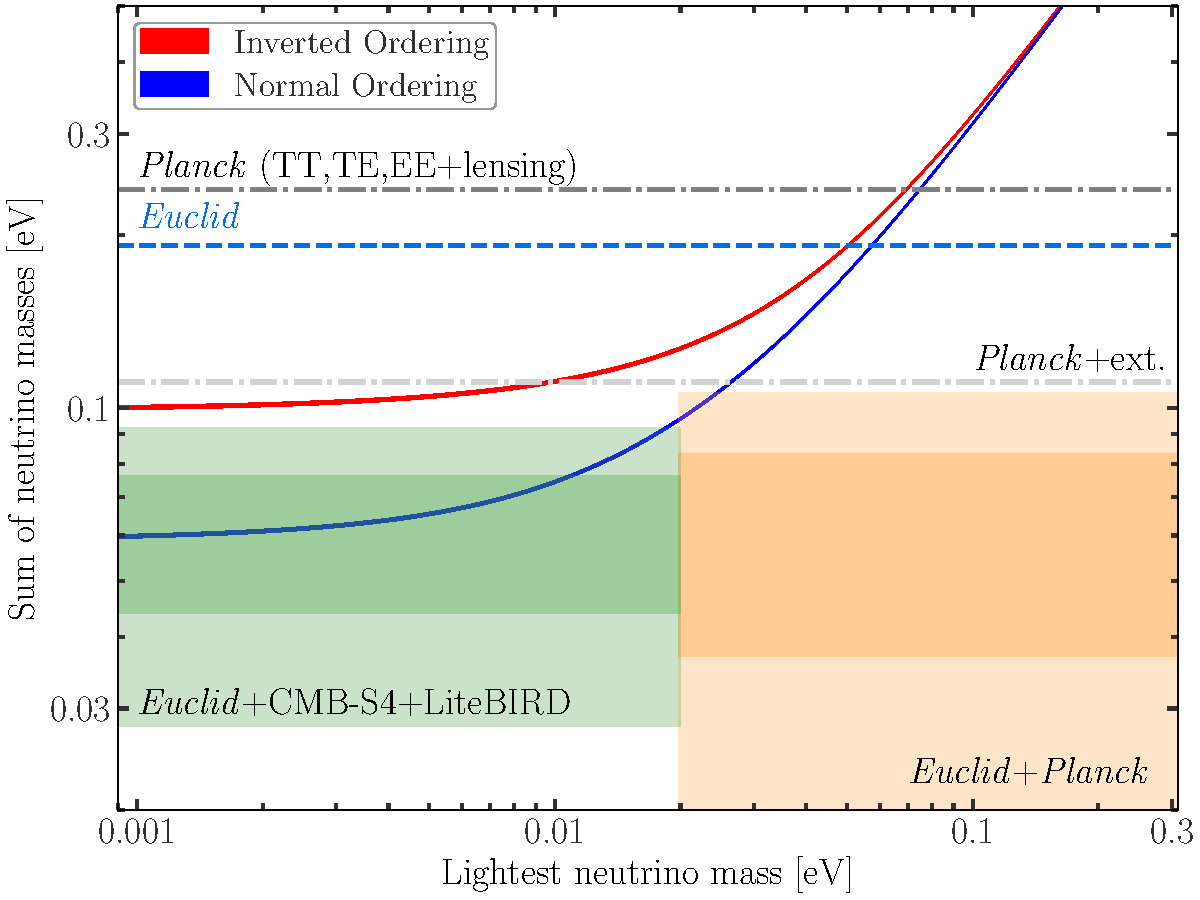
\includegraphics[width=\linewidth]{figure_hierarchy-1.pdf}
    \end{subfigure}
    \hfill
    \begin{subfigure}{0.49\textwidth}
        \centering
        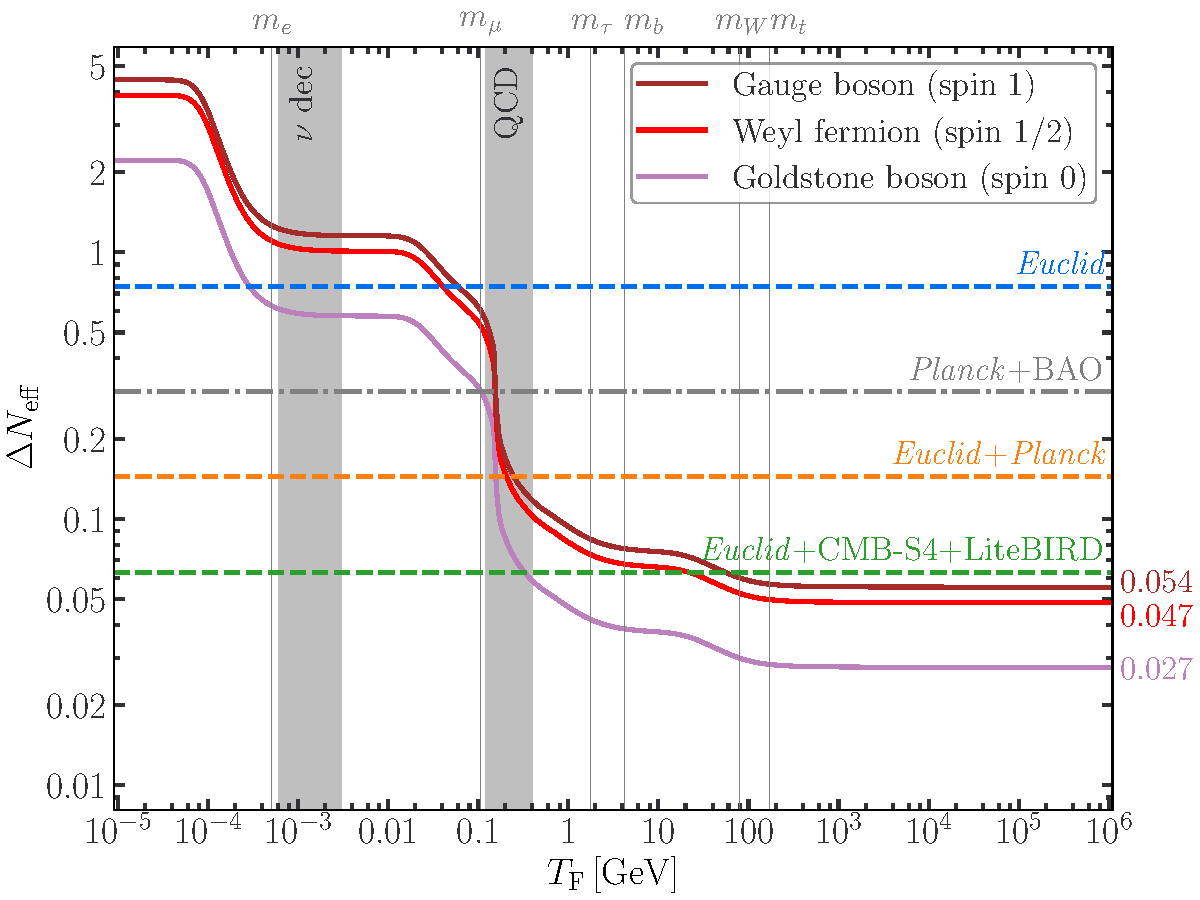
\includegraphics[width=\linewidth]{figure_Neff-1.pdf}
    \end{subfigure}
    \caption{\textit{left}, forecast sensitivity for the $\summnu$ for different combinations of \euclid with or without external CMB data. We compare the sensitivities to current measurements of \planck or \planck + additional data from supernovae, BAO measurements and current large scale structure measurements. The dashed lines represent the 95\% CL. The strike-through lines represent the sum of the neutrino masses from oscillation experiments depending on the ordering and the lowest neutrino mass.;\\
    \textit{right}, Similar to the left plot but for the sensitivity for $\dneff$. The strike-through lines represent contritubtions to $\dneff$ from different types of particles and different decoupling temperatures. 
    }
    \label{fig:results}
\end{figure}

\bibliographystyle{JHEP}
\bibliography{my-bib-database}

\end{document}
